\documentclass[11pt,a4paper]{article}

\usepackage[margin=1in]{geometry}
\usepackage{graphicx}
\usepackage{booktabs}
\usepackage{hyperref}
\usepackage{amsmath}
\usepackage{url}

\title{TDF Radial Reconstruction on a Preregistered Controlled SPARC Subset:\\
Holdout Validation, Failure Modes, and Sensitivity-Recovery Cases}
\author{Bahman Masarrat\\
Independent Researcher\\
\href{mailto:bmasarrat@gmail.com}{bmasarrat@gmail.com}}
\date{\today}

\begin{document}

\maketitle

\begin{abstract}
We benchmark a Time-Delay Field (TDF) radial reconstruction framework on a pre-registered,
controlled subset of SPARC rotation curves \cite{lelli2016sparc}. This is \emph{not}
full-SPARC validation: results apply to the expansion-20 cohort ($n{=}20$) and the nested
expansion-12 cohort ($n{=}12$). The primary model is \texttt{tdf\_3knot};
\texttt{tdf\_5knot} is a sensitivity/high-flexibility diagnostic only. We use train-only
even/odd holdout comparisons against NFW \cite{navarro1997} and MOND \cite{milgrom1983}
baselines at fixed canonical baryons and fixed $K_\tau$. In the pre-registered controlled expansion-20 cohort, the primary conservative \texttt{tdf\_3knot}\  model achieves robust holdout success in 15 of 20 galaxies. Three additional galaxies show sensitivity-recovery where \texttt{tdf\_5knot}\  improves substantially but is not counted as primary success. NGC7814 remains the only all-TDF holdout failure, and UGC00128 remains a mixed near-tie case. The analysis does not
disprove dark matter, does not replace $\Lambda$CDM, does not test lensing, claims no
universal $\tau$-profile, and makes no final $M/L$ calibration claim.
\end{abstract}

\section{Introduction}
Galaxy rotation curves provide a disciplined test of how well models reproduce observed
circular speeds beyond the baryonic contribution \cite{lelli2016sparc}. This paper is a
\emph{controlled benchmark} of TDF as a reconstruction framework---not a dark-matter-disproof
or $\Lambda$CDM-replacement study. Predictive holdout validation matters because in-sample
fits can reward extra flexibility; we therefore require \texttt{tdf\_3knot} to perform on
held-out radii against standard baselines before counting primary success. We extend an earlier six-galaxy pilot benchmark (repository history) that established an
explicit NGC7814 failure mode to pre-registered expansion-12 and expansion-20 cohorts with
frozen failure-mode taxonomy \cite{tdf_benchmark2026}.

Many rotation-curve studies optimize in-sample fit quality. Here we prioritize predictive
holdout consistency to reduce flexibility-driven overfitting \cite{geisser1975,arlot2010}.
We do not claim that holdout success ``proves'' TDF at cosmological level; it is a conservative
empirical gate on the controlled subset.

\section{TDF reconstruction framework}
TDF reconstructs a radial $\tau(r)$ from rotation-curve residuals relative to fixed SPARC
baryonic components \cite{lelli2016sparc,mcgaugh2016}.

\subsection{Benchmark definition}
We decompose the observed rotation curve into baryonic and TDF-mediated contributions,
\begin{equation}
  v_{\mathrm{obs}}^2(r) = v_{\mathrm{bar}}^2(r) + v_{\tau}^2(r),
  \label{eq:vobs}
\end{equation}
with fixed catalog baryons $v_{\mathrm{bar}}^2 = v_{\mathrm{gas}}^2 + v_{\mathrm{disk}}^2 + v_{\mathrm{bulge}}^2$.
The TDF closure used in this benchmark is
\begin{equation}
  v_{\tau}^2(r) = r\, K_{\tau}\,\frac{d\tau}{dr},
  \label{eq:vtau}
\end{equation}
where $K_{\tau}$ is a fixed dimensionless coupling held constant across the cohort in the primary
analysis. Given $v_{\mathrm{obs}}(r)$ and $v_{\mathrm{bar}}(r)$, the direct reconstruction law is
\begin{equation}
  \frac{d\tau}{dr} = \frac{v_{\mathrm{obs}}^2(r) - v_{\mathrm{bar}}^2(r)}{r\, K_{\tau}}.
  \label{eq:dtaudr}
\end{equation}
Equation~(\ref{eq:dtaudr}) defines a \emph{galaxy-specific} $\tau(r)$ profile for each system.
The algebraic reconstruction law is universal; we do \textbf{not} claim a universal functional
$\tau(r)$ shape across galaxies. Repository diagnostic pointwise reconstruction from
Eq.~(\ref{eq:dtaudr}) is not used as a primary fitted competitor.

\subsection{Fitted knot regularization}
Fitted models (\texttt{tdf\_3knot}, \texttt{tdf\_5knot}) are low-parameter piecewise-linear
regularizations of $d\tau/dr$ with knot amplitudes optimized on training radii during holdout
evaluation. \texttt{tdf\_3knot} is the \textbf{primary conservative} parameterization;
\texttt{tdf\_5knot} increases flexibility and is reported only as a sensitivity diagnostic.


\section{Controlled SPARC benchmark protocol}
The pipeline ingests SPARC \texttt{rotmod} data, applies the frozen expansion plan, reconstructs
$\tau$, fits NFW/Burkert/MOND baselines, fits TDF knot models, runs holdout validation, audits
failure modes, and reconciles claims (Figure~\ref{fig:workflow}). All expansion\_20 numbers
are taken from frozen pipeline outputs; this editing phase does not rerun fits or alter tables.


\begin{figure}[htbp]
  \centering
  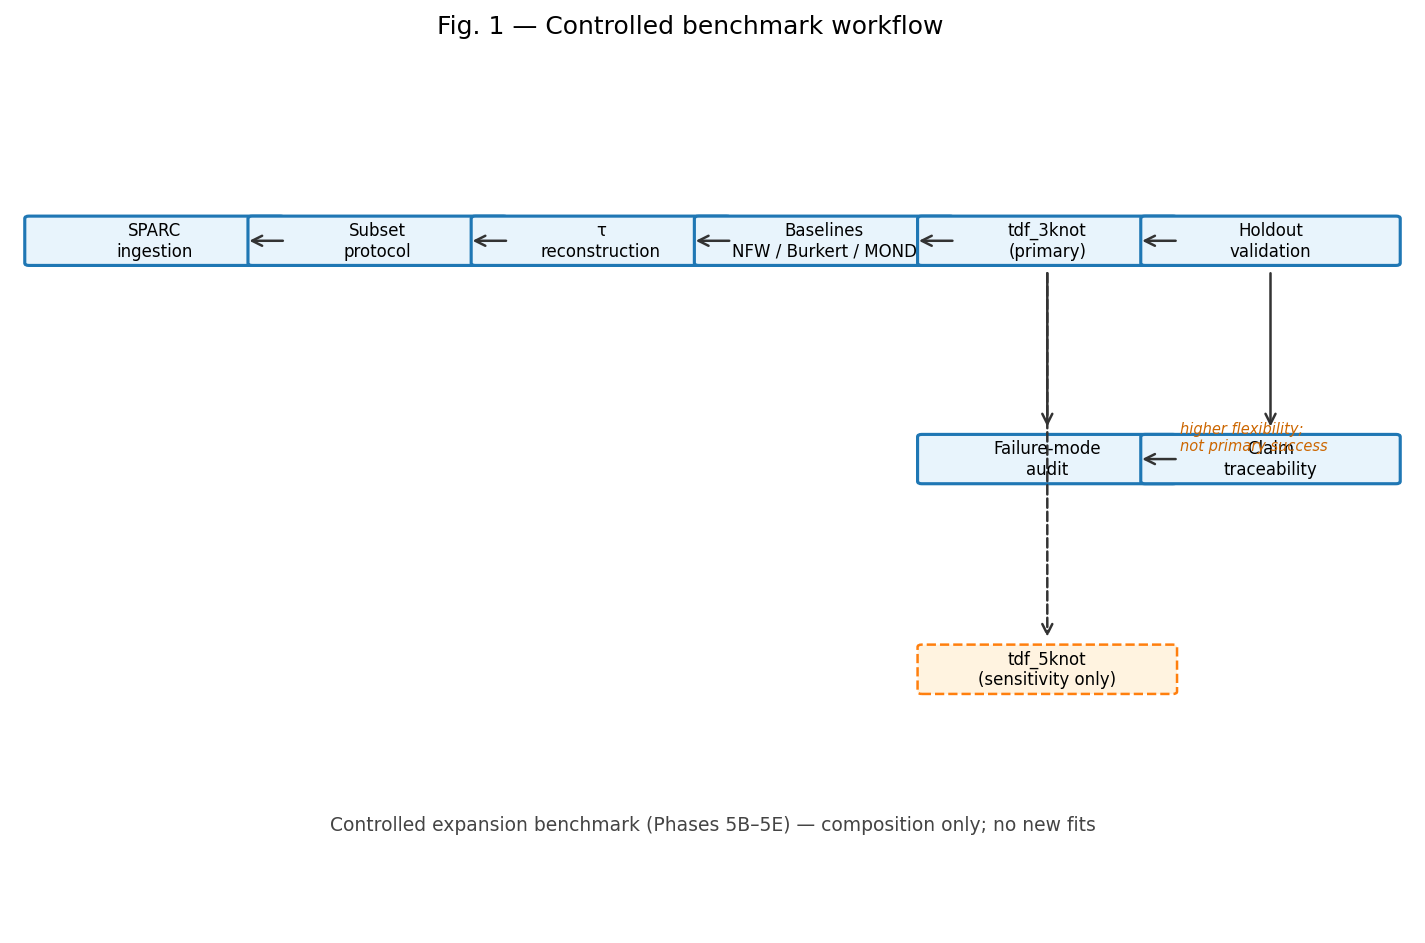
\includegraphics[width=\linewidth]{figures/fig1_benchmark_workflow.png}
  \caption{End-to-end benchmark workflow (ingestion through claim reconciliation).
  The solid path is the primary conservative pipeline (\texttt{tdf\_3knot}); the dashed
  branch is the high-flexibility sensitivity pipeline (\texttt{tdf\_5knot}), which is
  audited separately and excluded from primary success counts.}
  \label{fig:workflow}
\end{figure}


\section{Data and cohort selection}
Galaxies enter expansion\_20 in a pre-registered order (Table~\ref{tab:cohort}).
expansion\_12 is the nested twelve-galaxy subset used for intermediate auditing; expansion\_20
is the main reported cohort. Membership is fixed in \texttt{sparc\_subset\_expansion\_plan.csv}
with no post-hoc cherry-picking.

\begin{table}[htbp]
\centering
\caption{Pre-registered expansion\_20 cohort membership (Phase 5A plan).}
\label{tab:cohort}
\footnotesize
\begin{tabular}{llcc}
\toprule
Galaxy & Role & In expansion\_12 & Order \\
\midrule
DDO154 & original controlled six & Y & 1 \\
IC2574 & original controlled six & Y & 2 \\
NGC2403 & original controlled six & Y & 3 \\
NGC3198 & original controlled six & Y & 4 \\
NGC6503 & original controlled six & Y & 5 \\
NGC7814 & original controlled six & Y & 6 \\
UGC02953 & expansion addition & Y & 7 \\
UGC05253 & expansion addition & Y & 8 \\
UGC09133 & expansion addition & --- & 9 \\
UGC06787 & expansion addition & --- & 10 \\
NGC5055 & expansion addition & Y & 11 \\
UGC00128 & expansion addition & Y & 12 \\
NGC0289 & expansion addition & Y & 13 \\
UGC12506 & expansion addition & --- & 14 \\
UGC11455 & expansion addition & --- & 15 \\
NGC6015 & expansion addition & --- & 16 \\
DDO161 & expansion addition & Y & 17 \\
NGC7793 & expansion addition & --- & 18 \\
UGC07524 & expansion addition & --- & 19 \\
UGC08490 & expansion addition & --- & 20 \\
\bottomrule
\end{tabular}
\vspace{0.4em}
{\footnotesize
\par\noindent\textbf{Source:} \texttt{outputs/tables/sparc\_subset\_expansion\_plan.csv}.
\par\noindent\textbf{Caveat:} Controlled subset only; not full-SPARC validation.
\par
}
\end{table}


\section{Baseline models}
\subsection{Baryonic-only}
$v_{\mathrm{bar}}^2 = v_{\mathrm{gas}}^2 + v_{\mathrm{disk}}^2 + v_{\mathrm{bulge}}^2$
from catalog inputs without fitting $M/L$ in the primary benchmark.
\subsection{NFW and Burkert}
NFW \cite{navarro1997} and Burkert \cite{burkert1995} halos use log-space multistart refits;
boundary-limited solutions and high reduced $\chi^2$ may occur and should not be overinterpreted.
\subsection{MOND and RAR}
MOND \cite{milgrom1983,famaey2012} with fitted $a_0$ and optional RAR \cite{mcgaugh2016}
are empirical rotation-curve baselines only, not cosmological or lensing validations of MOND.

\paragraph{Burkert baseline scope.}
Burkert \cite{burkert1995} halos are implemented for completeness but are not emphasized in the
primary holdout gate because, under the frozen log-space multistart halo protocol, Burkert fits frequently exhibit
boundary-limited parameters and high reduced $\chi^2$ on this subset. NFW \cite{navarro1997} and
MOND \cite{milgrom1983,famaey2012} are the headline non-TDF comparators for
\texttt{robust\_tdf\_success}; Burkert results remain in pipeline tables for reproducibility.


\section{Holdout validation methodology}
\textbf{Primary split:} even/odd index holdout with train-only refit. \textbf{Classification
definitions (expansion\_20):}
\begin{itemize}
  \item \textbf{robust\_tdf\_success:} \texttt{tdf\_3knot} beats both NFW refit and MOND
  fit-$a_0$ on even/odd holdout RMSE (primary success).
  \item \textbf{sensitivity\_recovery:} \texttt{tdf\_3knot} fails the primary gate but
  \texttt{tdf\_5knot} improves substantially (not primary success).
  \item \textbf{tdf\_failure\_mode:} all TDF knot variants fail the primary holdout gate
  (NGC7814).
  \item \textbf{mixed\_result:} near-tie among models without a clear primary win (UGC00128).
\end{itemize}
Additional splits (blocked radial thirds, $k$-fold) are diagnostic
\cite{stone1974,arlot2010}. Model parsimony is summarized with AIC/BIC in pipeline tables
\cite{akaike1974,schwarz1978}; the primary gate here is predictive holdout RMSE, not in-sample
information criteria alone. Table~\ref{tab:holdout-rmse} lists per-galaxy even/odd RMSE.

\begin{table}[htbp]
\centering
\caption{Even/odd holdout test RMSE [km/s] for expansion\_20 (train-only refit).}
\label{tab:holdout-rmse}
\scriptsize
\begin{tabular}{@{}l l r r r r@{}}
\toprule
Galaxy & Classification & \texttt{tdf\_3knot} & NFW & MOND & \texttt{tdf\_5knot} \\
\midrule
DDO154 & Robust TDF success & 2.03 & 3.56 & 3.98 & 1.44 \\
DDO161 & Robust TDF success & 0.72 & 3.87 & 6.55 & 0.78 \\
IC2574 & Robust TDF success & 2.98 & 6.39 & 6.29 & 1.73 \\
NGC0289 & Robust TDF success & 19.81 & 21.91 & 22.95 & 19.54 \\
NGC2403 & Robust TDF success & 8.66 & 9.76 & 14.24 & 3.44 \\
NGC3198 & Robust TDF success & 10.45 & 12.00 & 14.34 & 8.24 \\
NGC5055 & Sensitivity recovery & 142.86 & 56.87 & 55.37 & 19.56 \\
NGC6015 & Robust TDF success & 7.13 & 8.27 & 13.45 & 4.86 \\
NGC6503 & Robust TDF success & 9.33 & 10.14 & 12.39 & 4.90 \\
NGC7793 & Robust TDF success & 4.57 & 8.15 & 8.47 & 3.80 \\
NGC7814 & TDF failure mode & 155.80 & 24.89 & 27.85 & 113.25 \\
UGC00128 & Mixed result & 3.00 & 2.72 & 6.24 & 5.06 \\
UGC02953 & Robust TDF success & 37.80 & 41.40 & 44.21 & 26.25 \\
UGC05253 & Sensitivity recovery & 48.52 & 36.15 & 37.38 & 16.46 \\
UGC06787 & Robust TDF success & 38.29 & 38.58 & 43.09 & 30.78 \\
UGC07524 & Robust TDF success & 1.63 & 2.82 & 3.58 & 1.52 \\
UGC08490 & Robust TDF success & 1.13 & 1.57 & 1.82 & 1.15 \\
UGC09133 & Robust TDF success & 33.24 & 36.27 & 37.96 & 25.74 \\
UGC11455 & Robust TDF success & 15.81 & 39.35 & 39.40 & 15.97 \\
UGC12506 & Sensitivity recovery & 11.92 & 8.00 & 20.14 & 5.76 \\
\bottomrule
\end{tabular}
\vspace{0.4em}
{\footnotesize
\par\noindent\textbf{Source:} \texttt{expansion20\_failure\_mode\_summary.csv}.
\par\noindent\textbf{Caveat:} Primary gate uses \texttt{tdf\_3knot}; \texttt{tdf\_5knot} is sensitivity only.
\par
}
\end{table}


\subsection{Descriptive holdout statistics}
Descriptive summary (expansion\_20, even/odd holdout; not hypothesis testing): robust primary success: 15/20 (75\%; descriptive 95\% bootstrap interval $[55\%,\,90\%]$); sensitivity-recovery: 3/20 (15\%; descriptive 95\% bootstrap interval $[0\%,\,30\%]$); TDF failure: 1/20 (5\%; descriptive 95\% bootstrap interval $[0\%,\,15\%]$); mixed: 1/20 (5\%; descriptive 95\% bootstrap interval $[0\%,\,15\%]$). Primary beats NFW: 15/20 (75\%; descriptive 95\% bootstrap interval $[55\%,\,90\%]$); primary beats MOND: 17/20 (85\%; descriptive 95\% bootstrap interval $[70\%,\,100\%]$). Median $\Delta$RMSE $\equiv$ RMSE$_{\mathrm{3k}}$ $-$ RMSE$_{\mathrm{baseline}}$: $-1.17$\,km/s vs NFW (galaxy-level 2.5--97.5\% range $[-14.07,\,109.57]$\,km/s) and $-3.60$\,km/s vs MOND ($[-16.29,\,108.74]$\,km/s). Negative $\Delta$RMSE indicates lower primary TDF holdout error.
We report bootstrap percentile intervals for cohort fractions as \emph{descriptive} uncertainty
brackets only; they are not hypothesis tests and do not establish cosmological significance.

\section{Results}
\subsection{expansion\_20 (main cohort)}
In the pre-registered controlled expansion\_20 cohort, the primary conservative \texttt{tdf\_3knot}\  model achieves robust holdout success in 15 of 20 galaxies. Three additional galaxies show sensitivity-recovery where \texttt{tdf\_5knot}\  improves substantially but is not counted as primary success. NGC7814 remains the only all-TDF holdout failure, and UGC00128 remains a mixed near-tie case.
Table~\ref{tab:classification} summarizes cohort-level counts. Figure~\ref{fig:expansion-summary}
contrasts expansion\_12 and expansion\_20 classifications. Representative robust-success rotation
curves (subset examples only) appear in Figure~\ref{fig:successes}.

\begin{table}[htbp]
\centering
\caption{Classification and holdout comparison: expansion\_12 vs expansion\_20.}
\label{tab:classification}
\footnotesize
\begin{tabular}{@{}l r r p{4.5cm}@{}}
\toprule
Metric & expansion\_12 & expansion\_20 & Notes \\
\midrule
Cohort size & 12 & 20 & expansion\_12 ⊂ expansion\_20 (same original six + overlapping additions) \\
Robust TDF success (primary) & 8 & 15 & Primary conservative success (tdf\_3knot beats NFW and MOND on holdout for e20) \\
Sensitivity recovery & 0 & 3 & Phase 5C class; not counted as primary success in e20 \\
TDF failure mode & 2 & 1 & NGC7814 all-TDF failure in both cohorts \\
Mixed result & 2 & 1 & UGC00128 near-tie in both \\
Primary beats NFW (holdout) & 8 & 15 & even/odd holdout; train-only refit \\
Primary beats MOND (holdout) & 9 & 17 & Required for robust\_tdf\_success in expansion\_20 \\
\bottomrule
\end{tabular}
\vspace{0.4em}
{\footnotesize
\par\noindent\textbf{Source:} \texttt{controlled\_expansion\_comparison\_summary.csv}.
\par\noindent\textbf{Caveat:} Robust TDF success requires primary \texttt{tdf\_3knot} to beat both NFW and MOND on holdout.
\par
}
\end{table}



\begin{figure}[htbp]
  \centering
  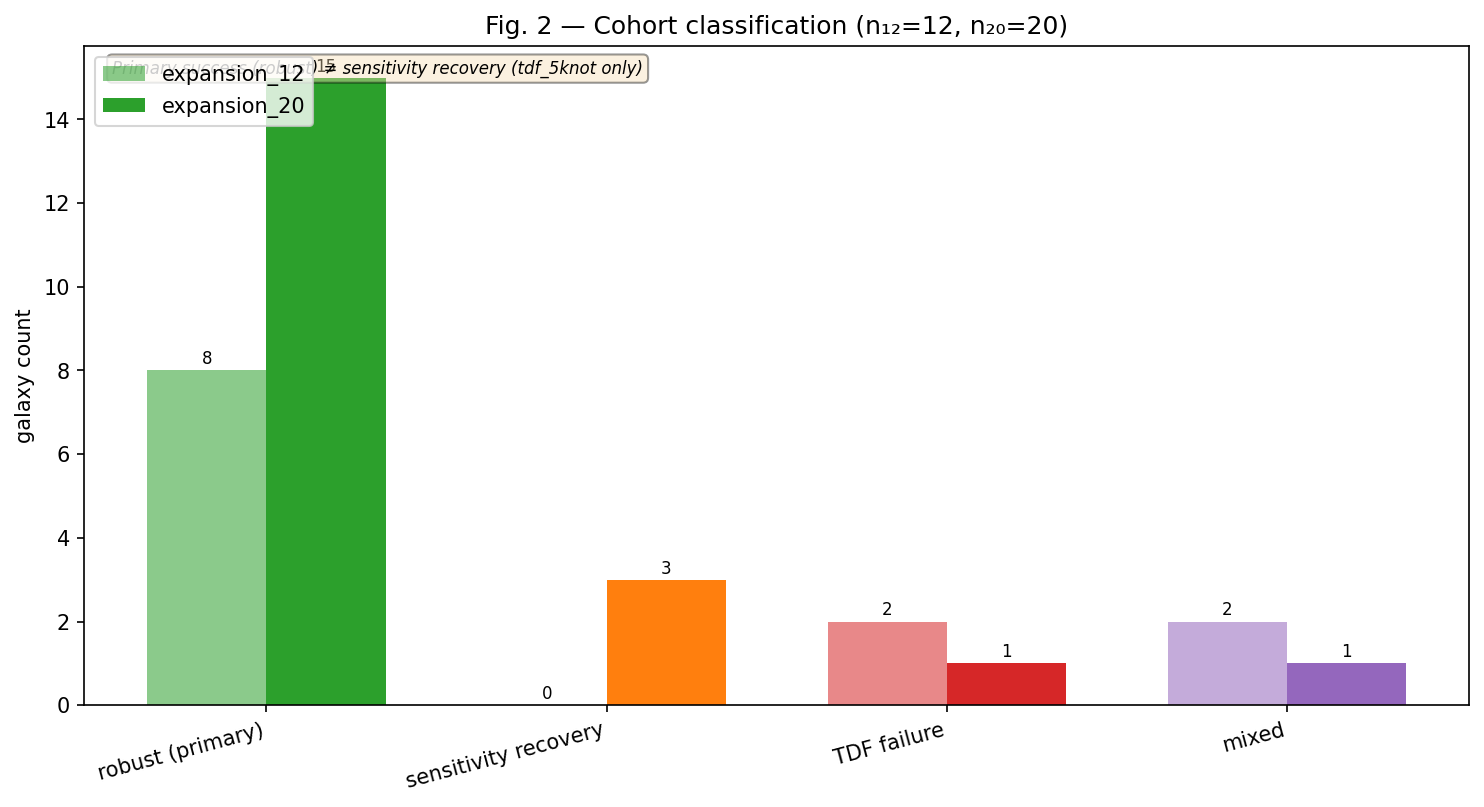
\includegraphics[width=0.92\linewidth]{figures/fig2_expansion12_vs_20_summary.png}
  \caption{Failure-mode counts for expansion-12 ($n{=}12$) and expansion-20
  ($n{=}20$). \textbf{Robust TDF success} (primary, \texttt{tdf\_3knot}) is shown separately
  from \textbf{sensitivity-recovery} (\texttt{tdf\_5knot} diagnostic only).}
  \label{fig:expansion-summary}
\end{figure}



\begin{figure}[htbp]
  \centering
  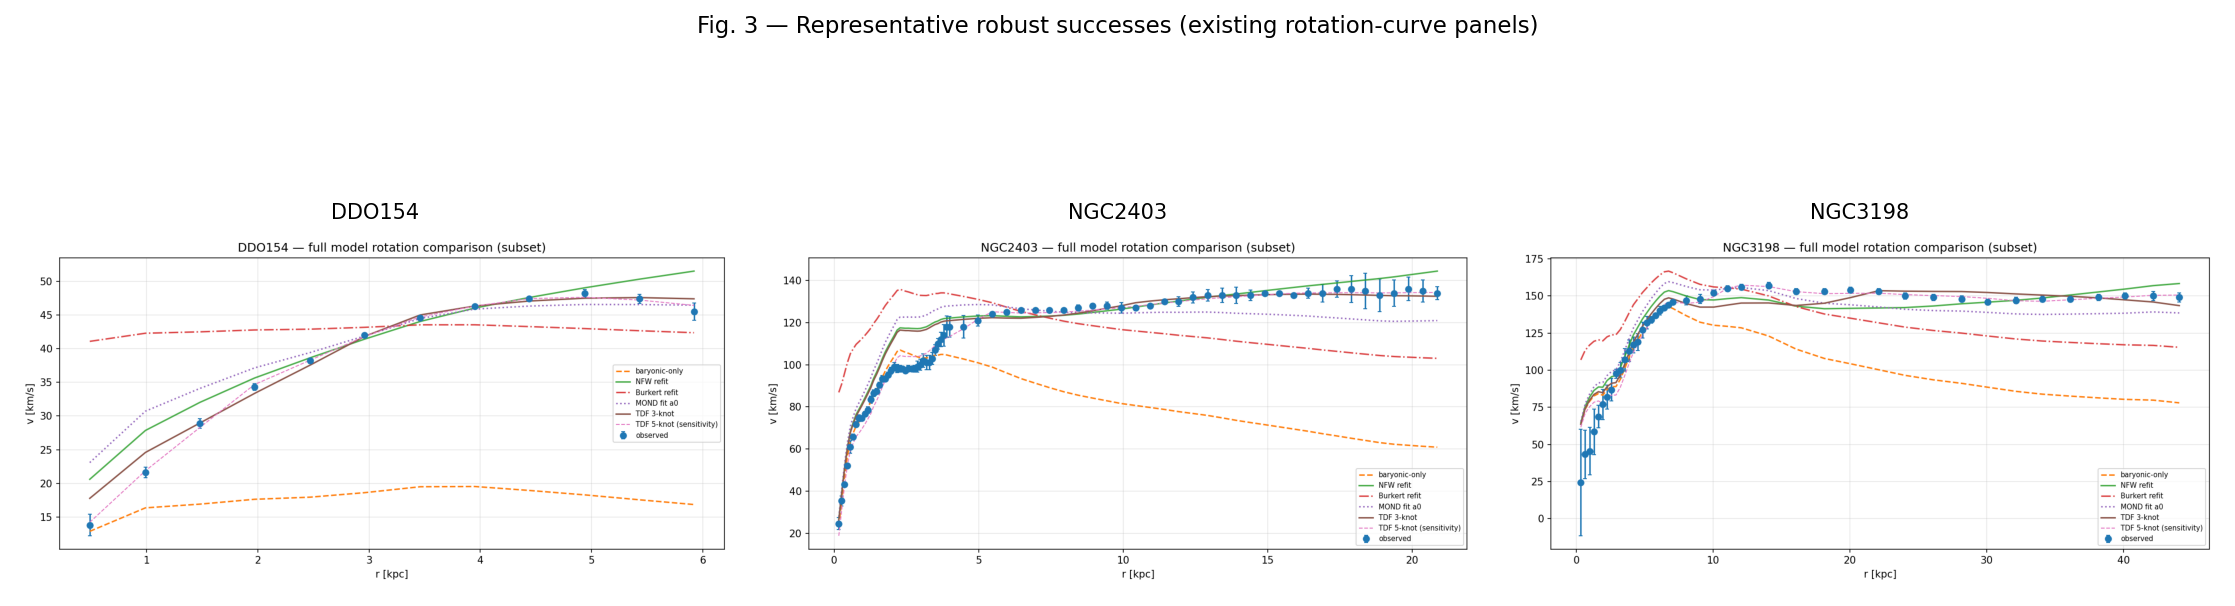
\includegraphics[width=\linewidth]{figures/fig3_representative_successes.png}
  \caption{Representative robust-success examples (DDO154, NGC2403, NGC3198). Panels are
  illustrative subset cases only, not a complete census of successes.}
  \label{fig:successes}
\end{figure}


\subsection{Primary success counts and Table~2 interpretation}
Primary success is defined only through \texttt{tdf\_3knot}: 15/20 robust successes. Seventeen
galaxies show \texttt{tdf\_3knot} beating MOND and fifteen beating NFW on even/odd holdout, but
robust success requires \textbf{both}. Table~\ref{tab:holdout-rmse} shows a heterogeneous
distribution: most robust-success galaxies exhibit primary RMSE at or below NFW/MOND, while
\textbf{NGC7814} is a decisive counterexample where all TDF variants remain poor on holdout
despite competitive in-sample flexibility. Three \texttt{sensitivity\_recovery} galaxies
(NGC5055, UGC05253, UGC12506) illustrate why \texttt{tdf\_5knot} is reported separately: large
holdout gains can reflect added knot freedom rather than validated primary-model superiority.
We do not extrapolate cohort fractions to the full SPARC catalog.

\subsection{expansion\_12 (nested context)}
expansion-12 ($n{=}12$) is a nested audit cohort: eight robust primary successes before
the expansion-20 taxonomy refinements (e.g.\ NGC5055 reclassified as sensitivity-recovery in
expansion-20). We report expansion-12 for continuity but treat expansion-20 as the main result.

\section{Failure modes and sensitivity recovery}
\textbf{NGC7814} remains the sole canonical all-TDF holdout failure (Figure~\ref{fig:ngc7814}).
\textbf{NGC5055}, \textbf{UGC05253}, and \textbf{UGC12506} exhibit sensitivity-recovery:
\texttt{tdf\_5knot} reduces holdout error markedly but these are \textbf{not} primary successes
(Figure~\ref{fig:sensitivity}). \textbf{UGC00128} is a mixed near-tie (NFW marginally best).
Per-galaxy holdout RMSE for all twenty galaxies is shown in Figure~\ref{fig:holdout-rmse}.
Table~\ref{tab:nonrobust} lists the five non-robust cases.

\begin{table}[htbp]
\centering
\caption{Non-robust expansion\_20 cases: holdout diagnostics (five galaxies).}
\label{tab:nonrobust}
\footnotesize
\begin{tabular}{@{}l l r r r@{}}
\toprule
Galaxy & Classification & RMSE$_{\mathrm{3k}}$ & RMSE$_{\mathrm{5k}}$ & $\Delta$RMSE [km/s] \\
\midrule
NGC7814 & TDF failure mode & 155.80 & 113.25 & 42.55 \\
NGC5055 & Sensitivity recovery & 142.86 & 19.56 & 123.31 \\
UGC05253 & Sensitivity recovery & 48.52 & 16.46 & 32.05 \\
UGC12506 & Sensitivity recovery & 11.92 & 5.76 & 6.16 \\
UGC00128 & Mixed result & 3.00 & 5.06 & -2.06 \\
\bottomrule
\end{tabular}
\vspace{0.4em}
{\footnotesize
\par\noindent\textbf{Source:} \texttt{expansion20\_failure\_diagnostics.csv}.
\par\noindent\textbf{Caveat:} Descriptive labels only; not causal claims about baryons or dark matter.
\par
}
\end{table}



\begin{figure}[htbp]
  \centering
  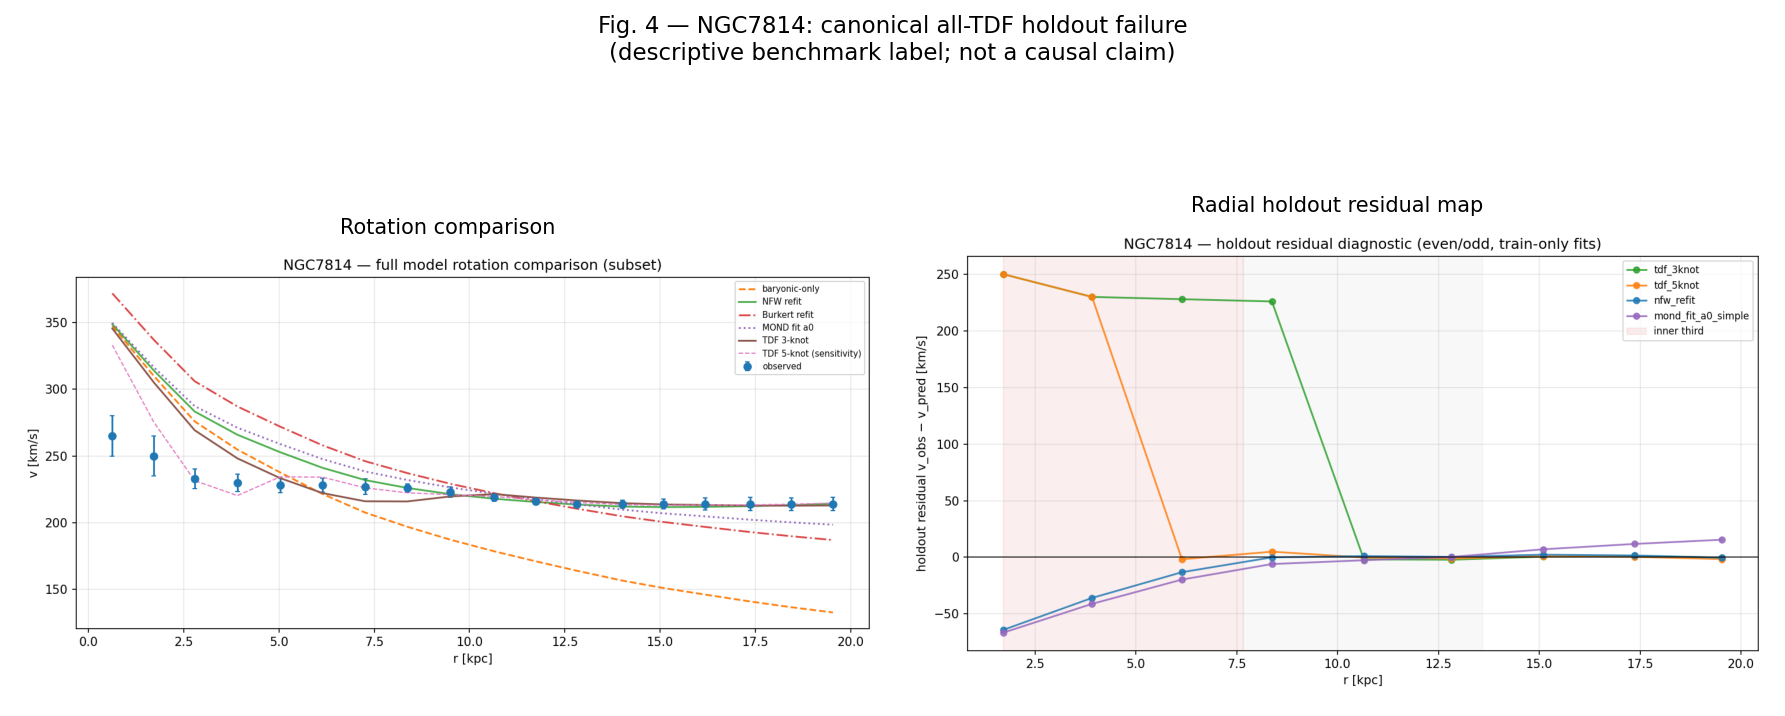
\includegraphics[width=\linewidth]{figures/fig4_ngc7814_failure.png}
  \caption{NGC7814 canonical all-TDF even/odd holdout failure. This is a
  \emph{descriptive} benchmark label for external reporting, not causal proof about
  baryons, halos, or dark matter.}
  \label{fig:ngc7814}
\end{figure}



\begin{figure}[htbp]
  \centering
  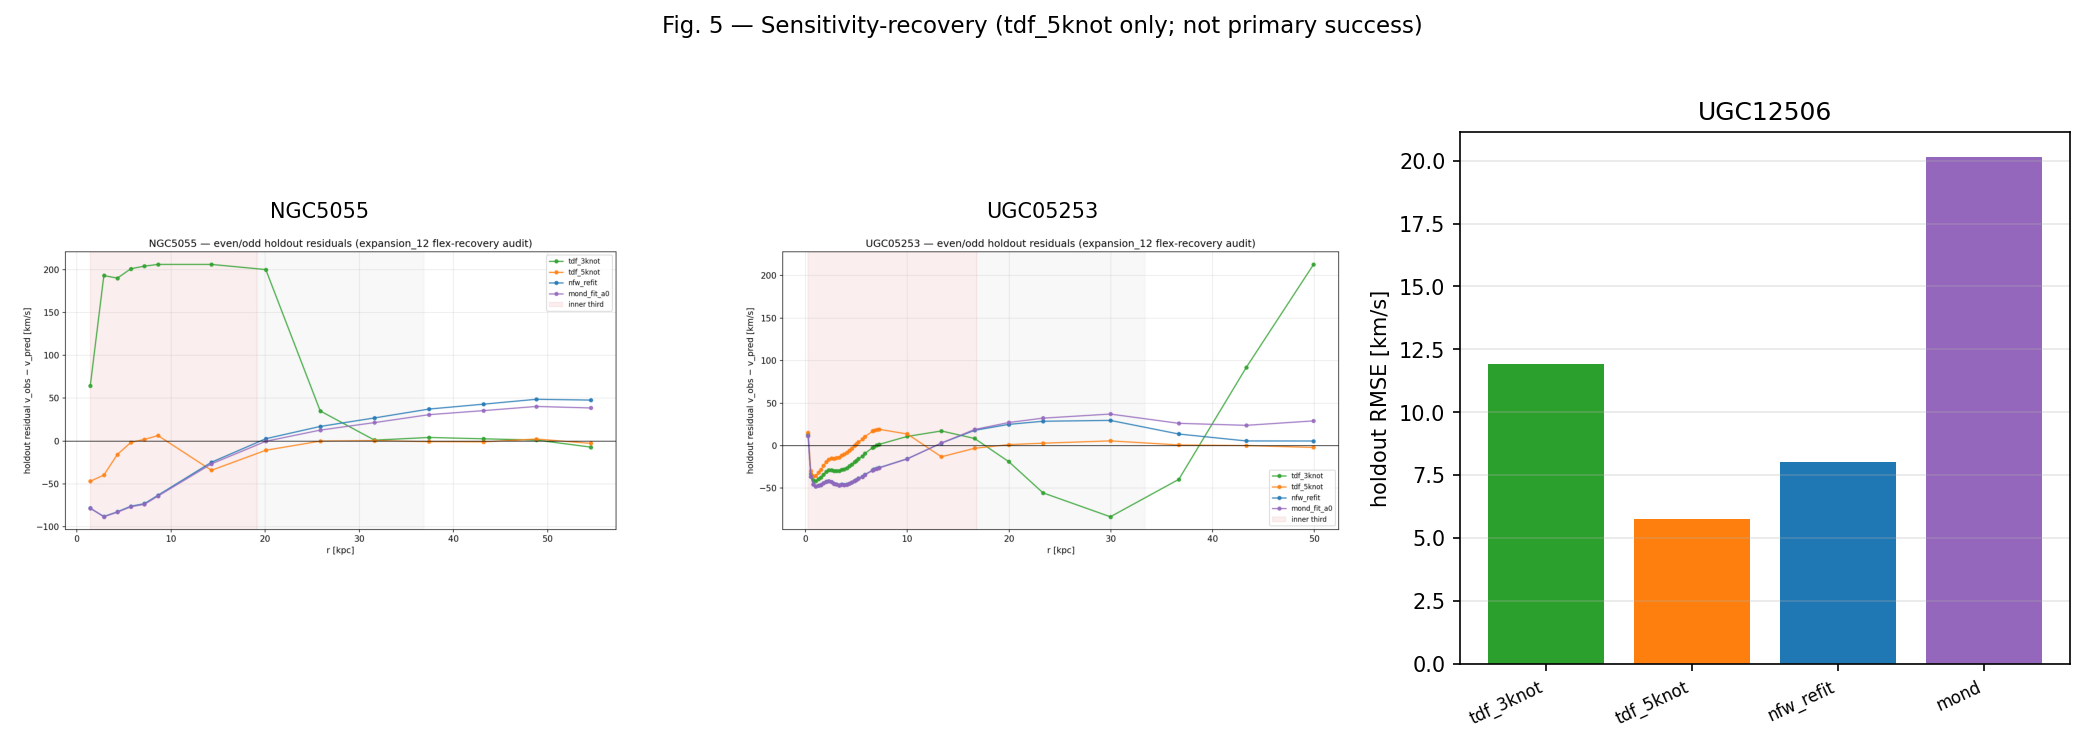
\includegraphics[width=\linewidth]{figures/fig5_sensitivity_recovery_cases.png}
  \caption{Sensitivity-recovery galaxies (NGC5055, UGC05253, UGC12506).
  Improved \texttt{tdf\_5knot} holdout performance is shown for diagnosis only and is
  \textbf{not} counted toward the 15/20 primary robust-success total.}
  \label{fig:sensitivity}
\end{figure}



\begin{figure}[htbp]
  \centering
  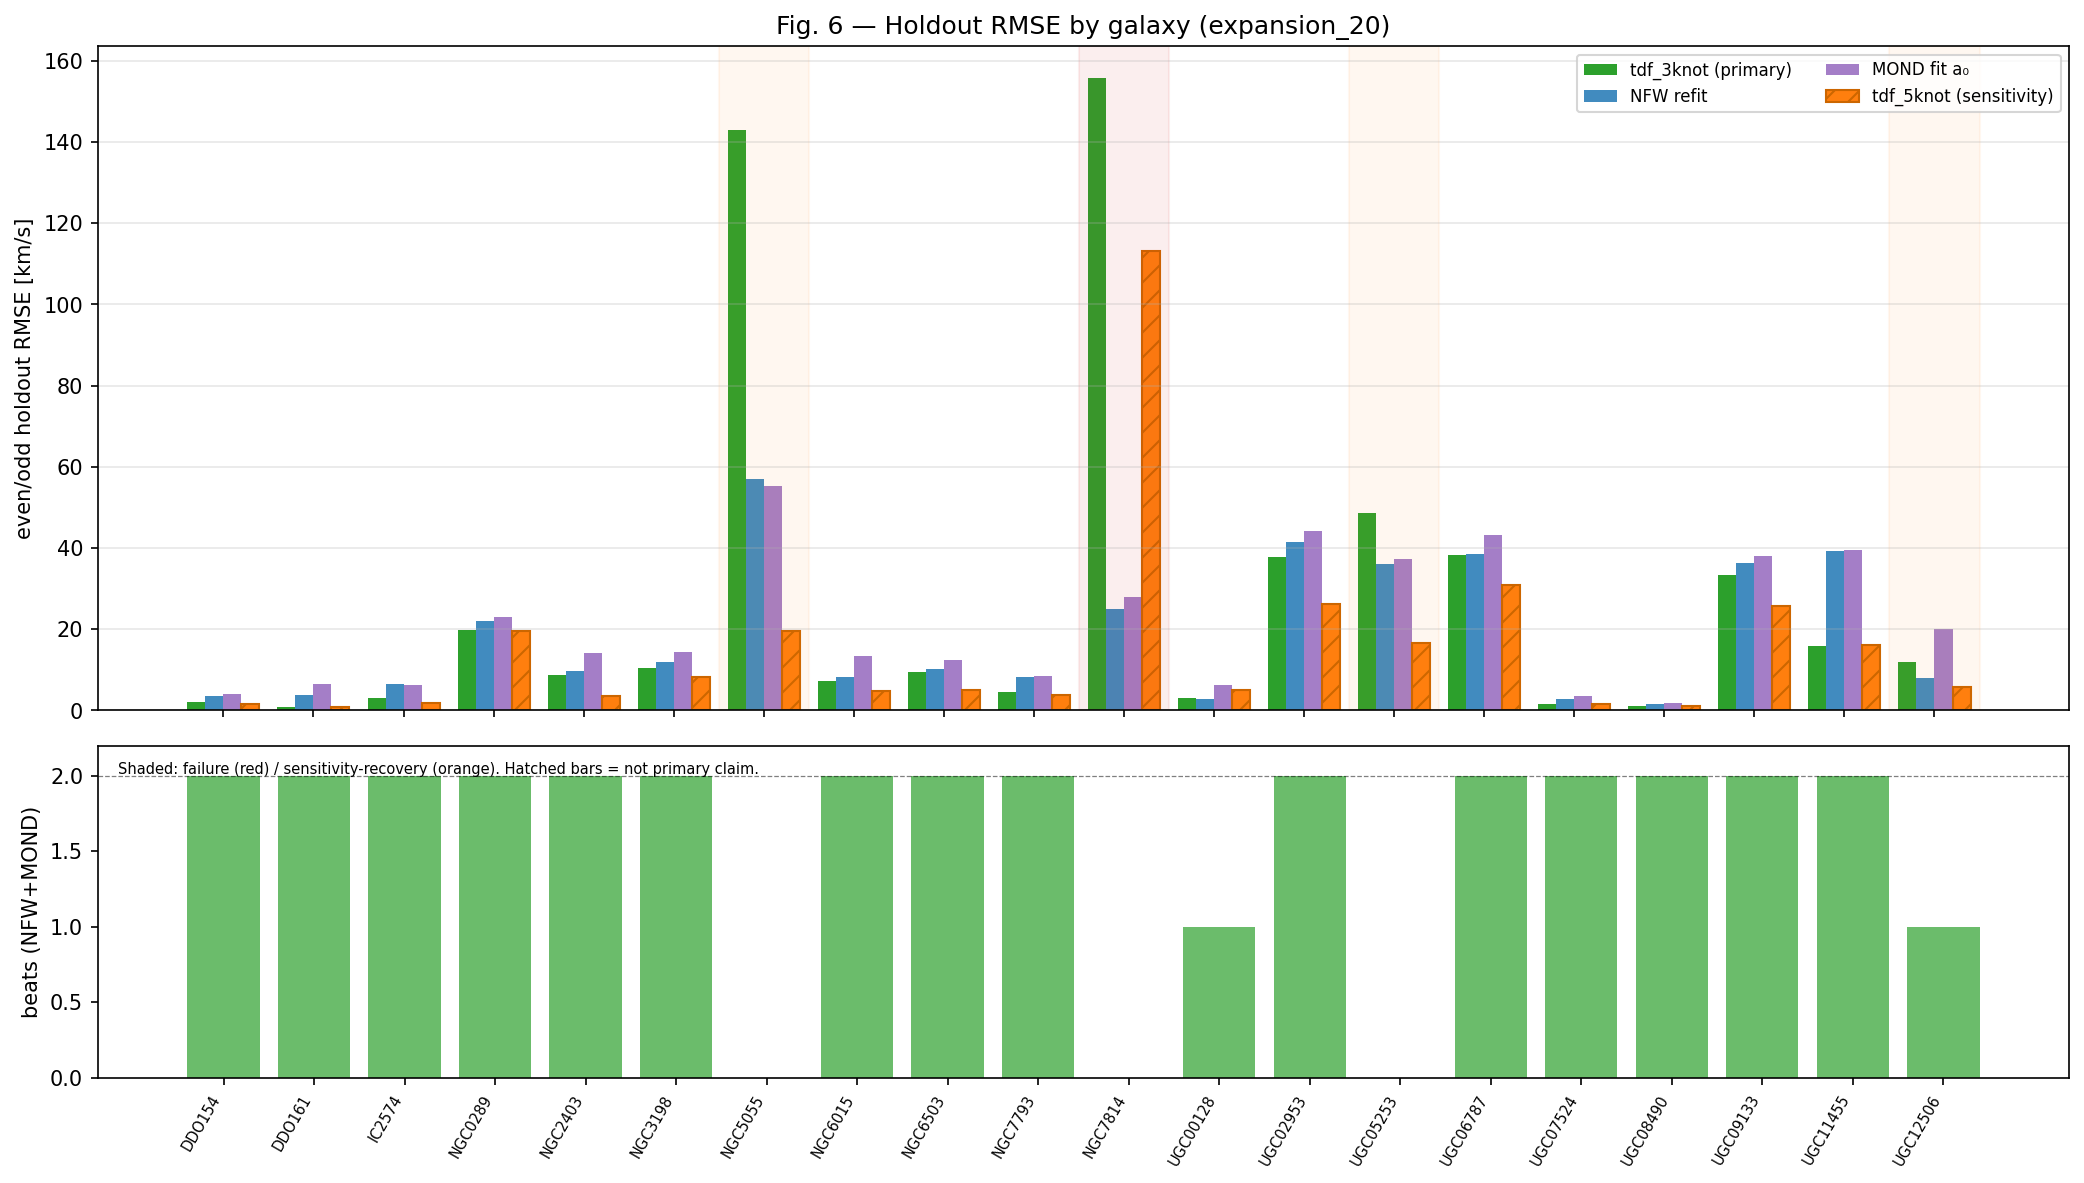
\includegraphics[width=\linewidth]{figures/fig6_holdout_rmse_comparison.png}
  \caption{Expansion-20 even/odd holdout RMSE by galaxy. Solid bars:
  \texttt{tdf\_3knot} (primary), NFW, and MOND; \textbf{hatched}
  \texttt{tdf\_5knot} bars are sensitivity-only and not used for primary claims.}
  \label{fig:holdout-rmse}
\end{figure}


\section{Limitations}
\begin{itemize}
  \item \textbf{Scope:} controlled expansion\_20 only---not full-SPARC validation.
  \item \textbf{Baryons and $M/L$:} fixed canonical decomposition; no final M/L calibration claim.
  \item \textbf{$K_\tau$:} held fixed in the benchmark; $K_\tau$ is not measured or inferred in this study.
  \item \textbf{Cosmology and lensing:} does not disprove dark matter; does not replace
  $\Lambda$CDM; lensing is not tested.
  \item \textbf{Flexibility:} \texttt{tdf\_5knot} carries higher overfitting/flexibility risk and
  is sensitivity-only.
  \item \textbf{$\tau$ universality:} per-galaxy diagnostics only; no universal $\tau$-profile claim.
\end{itemize}

\begin{table}[htbp]
\centering
\caption{Assumptions and limitations for the controlled expansion-20 manuscript.}
\label{tab:assumptions}
\footnotesize
\begin{tabular}{@{}p{0.48\linewidth}p{0.48\linewidth}@{}}
\toprule
\textbf{Assumptions (expansion-20)} & \textbf{Limitations (expansion-20)} \\
\midrule
$\bullet$ Benchmark scope is the pre-registered controlled expansion-20 cohort ($n{=}20$) only. & $\bullet$ Not full-SPARC validation; cohort fractions must not be extrapolated. \\
$\bullet$ Fixed canonical SPARC baryonic decomposition; no final $M/L$ calibration in this manuscript. & $\bullet$ Halo and MOND baselines remain degenerate with baryonic assumptions. \\
$\bullet$ $K_g$ is fixed across the cohort (legacy benchmark label $K_\tau$ in frozen tables); not measured or inferred; distinct from field stiffness $\kappa_\tau$. & $\bullet$ Higher knot count (\texttt{tdf\_5knot}) increases flexibility and overfitting risk. \\
$\bullet$ NFW and MOND are rotation-curve empirical baselines, not cosmology or lensing tests. & $\bullet$ Does not disprove dark matter and does not replace $\Lambda$CDM. \\
$\bullet$ Burkert halos are fitted for completeness but are not part of the primary holdout gate. & $\bullet$ Lensing is not tested in this benchmark phase. \\
$\bullet$ Primary model: \texttt{tdf\_3knot}; sensitivity model: \texttt{tdf\_5knot} (not primary success). & $\bullet$ No universal $\tau$-profile claim; per-galaxy $\tau$ diagnostics only. \\
$\bullet$ Even/odd train-only holdout is the primary predictive gate. & $\bullet$ Bootstrap intervals in the manuscript are descriptive, not significance tests. \\
\bottomrule
\end{tabular}
\vspace{0.4em}
{\footnotesize
\par\noindent\textbf{Source:} Phase~5F-F expansion-20 checklist (replaces legacy six-galaxy assumption bullets).
\par\noindent\textbf{Caveat:} Aligned with claims C20-A--C20-H; no change to frozen benchmark metrics.
\par
}
\end{table}


\section{Future work}
Full-catalog processing, lensing tests, two-dimensional $\tau$ maps, and photometry-calibrated
$M/L$ priors require protocol amendments. Blocked-holdout maps for UGC12506 may localize radial
failure without changing frozen primary labels.

\section{Conclusion}
On the pre-registered controlled expansion\_20 subset, \texttt{tdf\_3knot} achieves robust
even/odd holdout success in 15 of 20 galaxies at fixed baryons and $K_\tau$, with three
sensitivity-recovery cases, one all-TDF failure (NGC7814), and one mixed near-tie (UGC00128).
TDF is a benchmarked reconstruction framework within explicit claim boundaries, not a
cosmology-replacement or dark-matter-disproof result.

\appendix
\section{Reproducibility appendix}
Benchmark: \texttt{python3 scripts/run\_expansion20\_pipeline.py}; audit:
\texttt{python3 scripts/build\_controlled\_expansion\_final\_audit.py}; tables:
\texttt{python3 scripts/export\_paper\_tables.py}; figures:
\texttt{python3 scripts/build\_paper\_figures.py}; PDF:
\texttt{python3 scripts/compile\_paper\_pdf.py}. Repository: \cite{tdf_benchmark2026}.

\section{Claim-boundary appendix}
Table~\ref{tab:claims-matrix} and Figure~\ref{fig:claims} document claims C20-A--C20-H.
Prohibited external language includes full-SPARC validation, dark-matter disproof, $\Lambda$CDM
replacement, lensing confirmation, and universal $\tau$-profile discovery.

\begin{table}[htbp]
\centering
\caption{Claim traceability matrix for controlled expansion\_20 (C20-A--C20-H).}
\label{tab:claims-matrix}
\scriptsize
\begin{tabular}{@{}p{1.1cm} p{10.2cm} p{2.8cm}@{}}
\toprule
ID & Claim & Status \\
\midrule
C20-A & expansion\_20 cohort processed reproducibly through frozen pipeline. & Supported \\
C20-B & Primary tdf\_3knot robust holdout success in 15 of 20 galaxies. & Supported (caveat) \\
C20-C & tdf\_5knot improves sensitivity-recovery cases. & Sensitivity only \\
C20-D & NGC7814 remains all-TDF holdout failure. & Supported \\
C20-E & TDF validated on full SPARC. & Not supported \\
C20-F & Dark matter is disproven. & Prohibited \\
C20-G & Lensing confirms TDF. & Not tested \\
C20-H & Universal τ-profile discovered. & Not supported \\
\bottomrule
\end{tabular}
\vspace{0.4em}
{\footnotesize
\par\noindent\textbf{Source:} \texttt{controlled\_expansion\_final\_claims.csv}.
\par\noindent\textbf{Caveat:} Authoritative language boundary for external reporting.
\par
}
\end{table}



\begin{figure}[htbp]
  \centering
  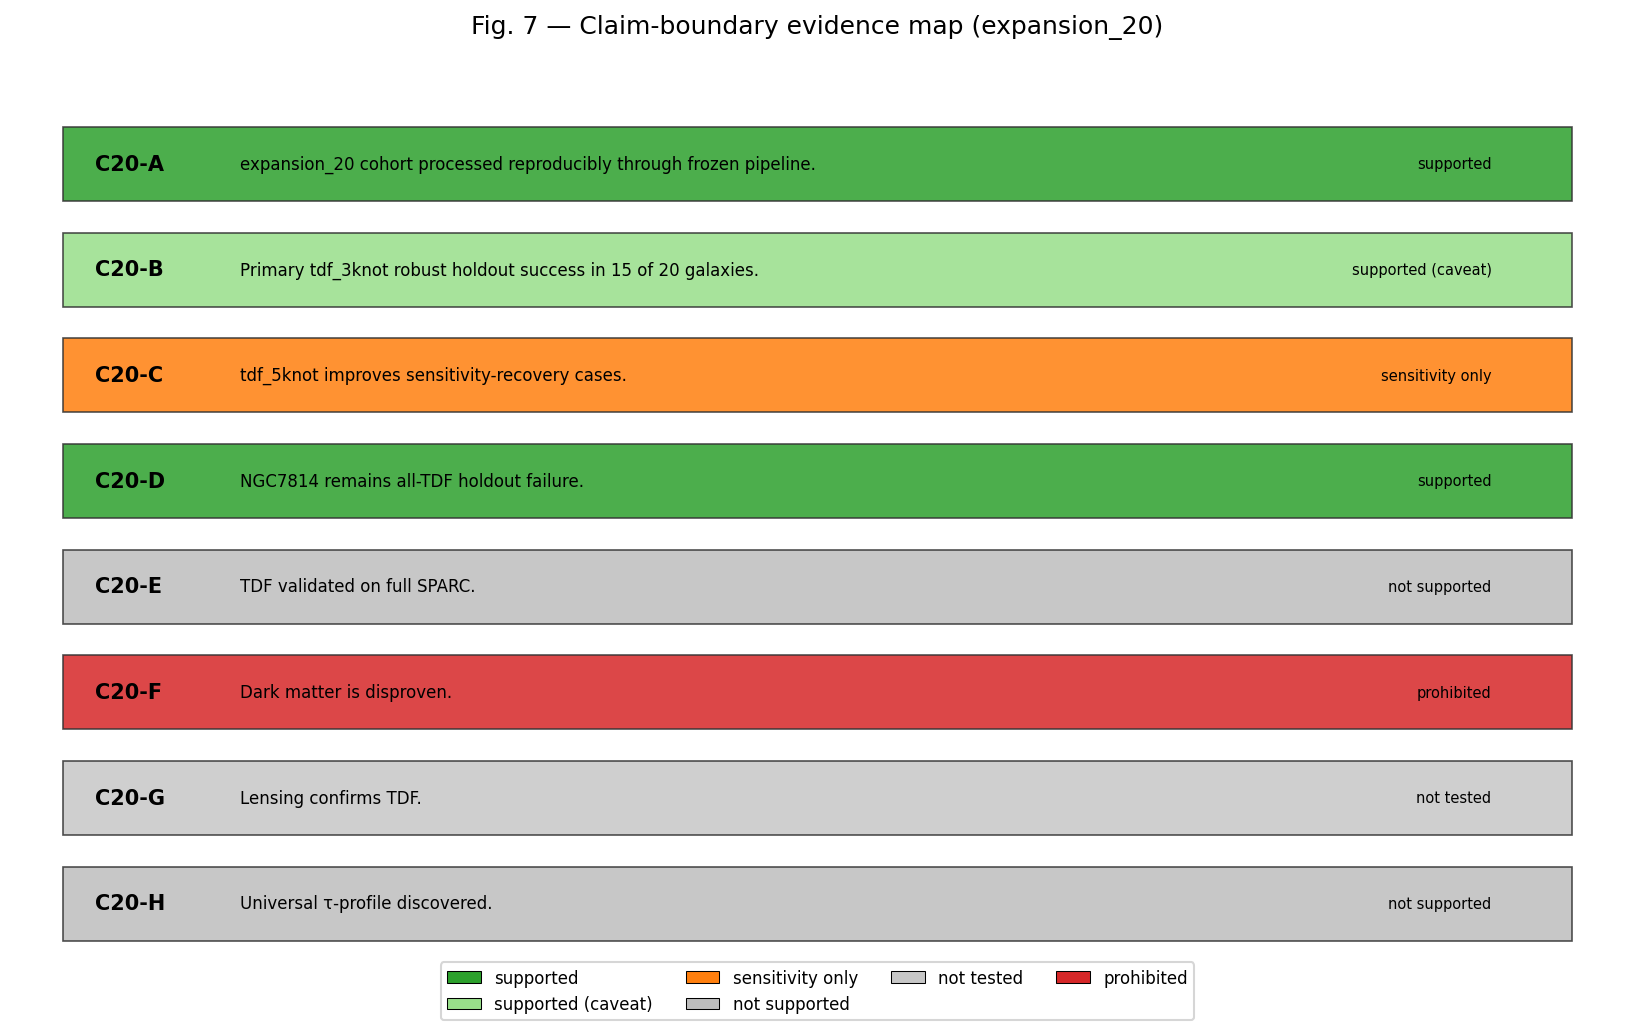
\includegraphics[width=0.95\linewidth]{figures/fig7_claim_boundary_map.png}
  \caption{External claim-boundary map for audited claims C20-A--C20-H (supported,
  caveat, sensitivity-only, not supported, prohibited).}
  \label{fig:claims}
\end{figure}


\bibliographystyle{plain}
\bibliography{references}

\end{document}
